\section{Introduction to Django}
% \subsection{Flowchart}


\begin{frame}[c]{Django is a Popular Framework}
    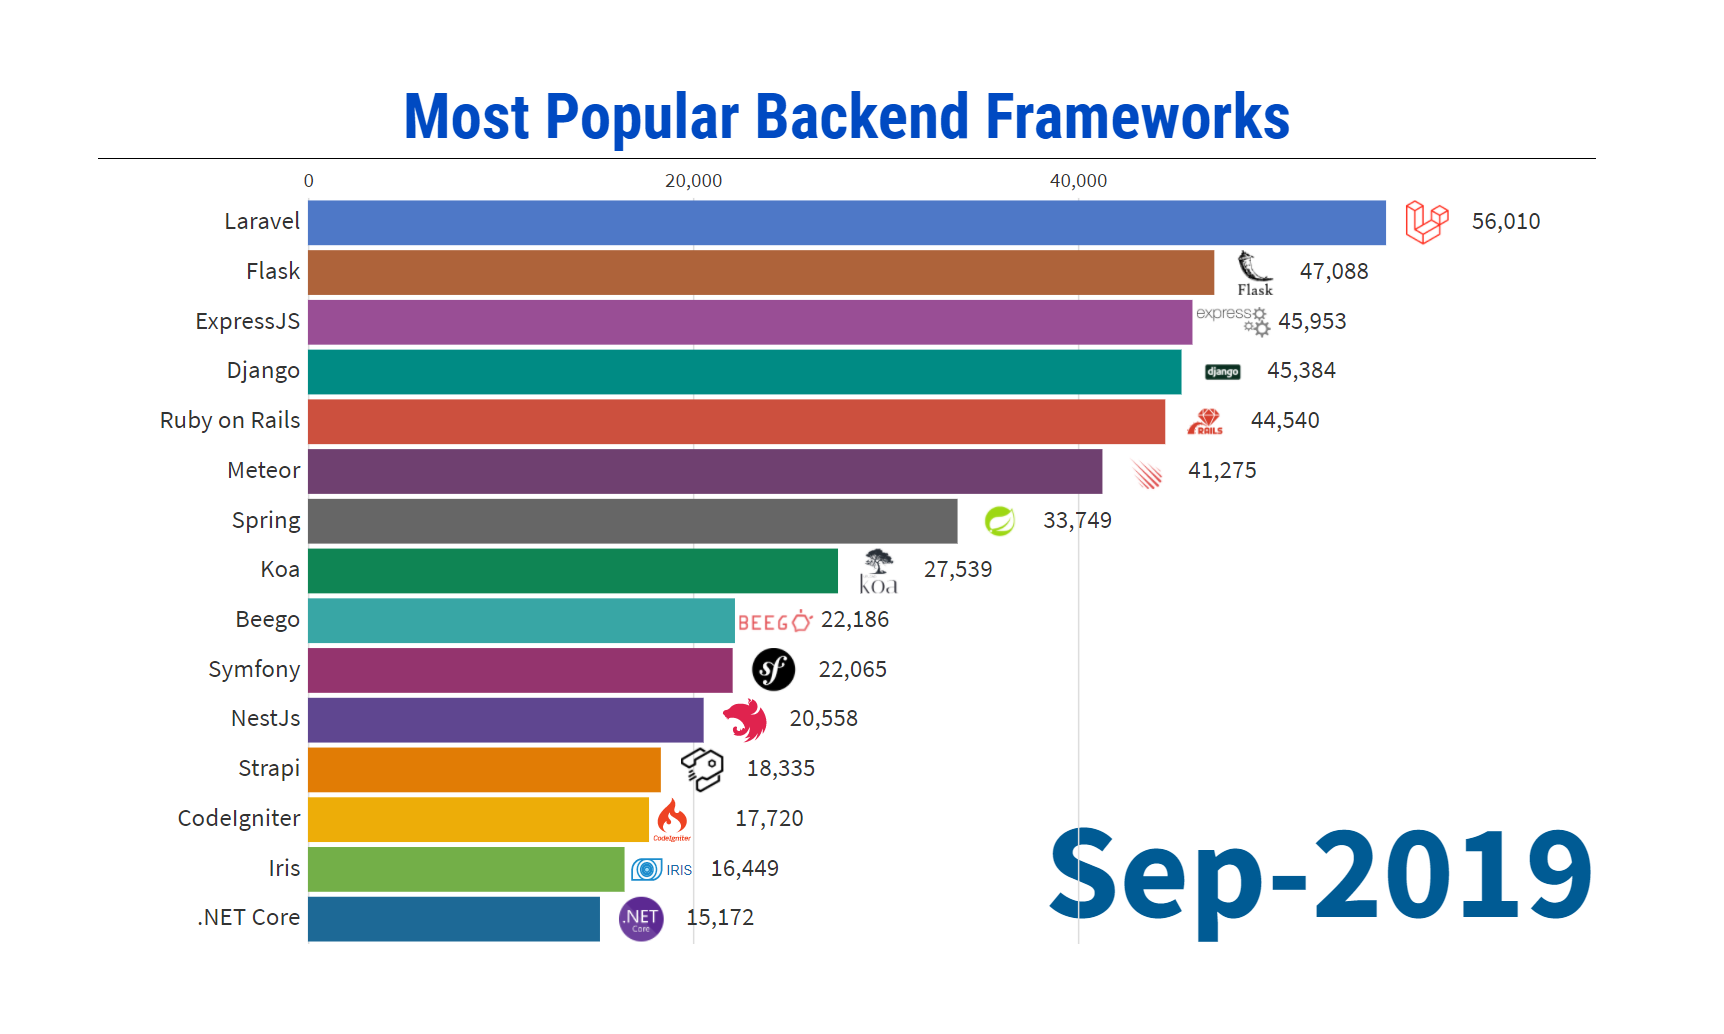
\includegraphics[width=0.9\textwidth,trim=0 60 0 50,clip]{backend_frameworks} \\
    Image source: \cite{frameworks}
    % Source: https://statisticsanddata.org/data/most-popular-backend-frameworks-2012-2021/
\end{frame}

\pic{What is Django?}{30}

\begin{frame}{Django Overview}
    % Image of entrypoint to view to form to model and stuff
    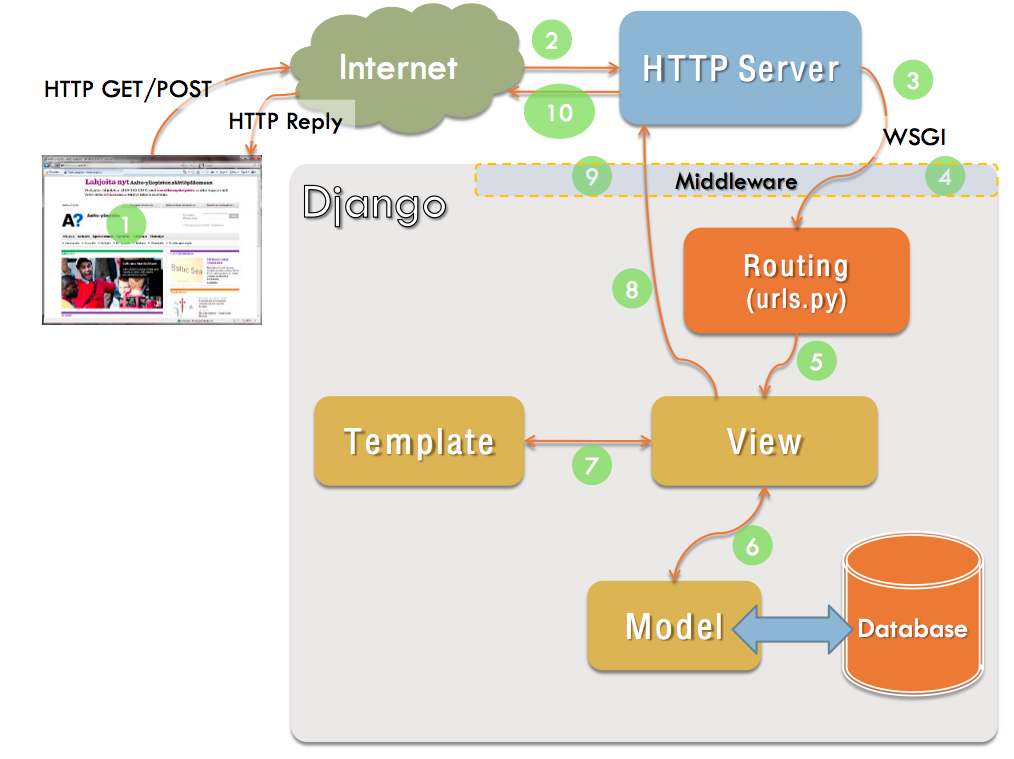
\includegraphics[height=0.9\textheight]{django_overview}
    Image source: \cite{overview}
    % Source: http://lectures.webcourse.niksula.hut.fi/img/django_mtv.png
\end{frame}


% \begin{frame}[c]{Django Changes to Models}
%     Quickly introduce model changes to seemless migrations
%     \begin{itemize}[<+(1)->]
%         \item Changes to ORM (Object Relational Mapping) result in `migrations`
%         \item Migrations can be applied and rolled back at any time
%     \end{itemize}
% \end{frame}

% \subsection{Commonly used terms}
% 
% 
% \begin{frame}[c]
%     Not sure if / what to put here?
% \end{frame}

